\documentclass[a4paper,12pt]{report}
\usepackage{graphicx}
\usepackage{sectsty}
\chapterfont{\Large\centering\MakeUppercase}
\usepackage{amsmath,amssymb}
\usepackage{setspace}
\onehalfspacing
\usepackage{array}
\usepackage{tikz}
\usetikzlibrary{shapes,arrows.meta,positioning,fit,calc}
\usepackage{listings}
\usepackage{xcolor}
\usepackage{url}
\usepackage{hyperref}
\hypersetup{
    colorlinks=false,
    pdfborder={0 0 0},
}

% Page Setup: A4, Left=3cm, Right=2.5cm, Top=2.5cm, Bottom=2.5cm, Headheight=15pt
\usepackage[top=2.5cm,bottom=2.5cm,left=3.0cm,right=2.5cm,headheight=15pt]{geometry}

% Header and Footer setup (Fancyhdr)
\usepackage{fancyhdr}
\pagestyle{fancy}
\fancyhf{}
\rhead{\nouppercase{\textit{\leftmark}}}
\lfoot{\textit{Department of CSE, Amal Jyothi College of Engineering}}
\rfoot{\textit{\thepage}}
\renewcommand{\headrulewidth}{0.4pt}
\renewcommand{\footrulewidth}{0.4pt}

\begin{document}

% 1. Title Page (No page number)
\begin{titlepage}
\begin{center}

{\Large \textbf{MULTIMODAL PHISHING WEBSITE\\ DETECTION USING EXPLAINABLE\\ ARTIFICIAL INTELLIGENCE}}\\[1.0cm]

\normalsize
\textbf{A SEMINAR REPORT}\\[0.2cm]
\textit{submitted by}\\[0.5cm]

{\large \textbf{ABIN BIJU JOSEPH}}\\[0.15cm]
\textbf{AJC23CS006}\\[0.6cm]

\textit{to}\\[0.4cm]
the \textbf{APJ Abdul Kalam Technological University}\\[0.15cm]
\textit{in partial fulfillment of the requirement for the award of the Degree of}\\[0.3cm]

\textbf{\large Bachelor of Technology}\\[0.15cm]
\textit{in}\\[0.15cm]
\textbf{\large Computer Science and Engineering}\\[0.8cm]

\textit{Under the guidance of}\\[0.2cm]
{\large \textbf{Prof. Lida K. Kuriakose}}\\[0.1cm]
\textbf{Assistant Professor}\\[0.8cm]


\includegraphics[width=0.25\textwidth]{ajcelogo2023.png}\\[0.5cm]

{\large \textbf{Department of Computer Science and Engineering}}\\[0.15cm]
{\large \textbf{Amal Jyothi College of Engineering (Autonomous)}}\\[0.15cm]
\textbf{Kanjirappally -- 686518}\\[0.5cm]

{\large \textbf{October 2026}}

\end{center}
\end{titlepage}


% 2. Certificate Page (No page number)
\begin{titlepage}
\begin{center}
{\large \textbf{DEPARTMENT OF COMPUTER SCIENCE AND ENGINEERING}}\\[0.15cm]
{\large \textbf{AMAL JYOTHI COLLEGE OF ENGINEERING (AUTONOMOUS)}}\\[0.15cm]
\textbf{KANJIRAPPALLY -- 686518}\\[0.5cm]


\includegraphics[width=0.25\textwidth]{ajcelogo2023.png}\\[0.4cm]

{\Large \textbf{CERTIFICATE}}\\[0.4cm]
\end{center}

\normalsize
\begin{spacing}{1.5}
\noindent This is to certify that the seminar report entitled \textbf{``Multimodal Phishing Website Detection Using Explainable Artificial Intelligence''} submitted by \textbf{ABIN BIJU JOSEPH (AJC23CS006)} to the APJ Abdul Kalam Technological University in partial fulfillment of the requirements for the award of the Degree of Bachelor of Technology in Computer Science and Engineering during the year 2026--2027, is a bonafide work carried out by him under my guidance and supervision.
\end{spacing}

\vspace{1.8cm}

\noindent
\begin{tabular*}{\textwidth}{@{\extracolsep{\fill}}lr}
\textbf{Prof. Lida K. Kuriakose} & \textbf{Dr. Anju J Prakash \quad Ms. Shiney Thomas} \\
Internal Supervisor & Seminar Coordinators \\
Assistant Professor &
\end{tabular*}

\vspace{1.5cm}

\begin{center}
\textbf{Dr. Juby Mathew}\\
Head of Department, CSE
\end{center}

\end{titlepage}


% Front Matter (Roman numerals starting at i for Acknowledgement)
\pagenumbering{roman}
\pagestyle{plain}
\setcounter{page}{1}

% 4. Acknowledgement (Page i)
\chapter*{ACKNOWLEDGEMENT}
\addcontentsline{toc}{chapter}{ACKNOWLEDGEMENT}

\begin{spacing}{1.5}
First of all, I sincerely thank the \textbf{Almighty GOD} who is most beneficent and merciful for granting me wisdom, endurance, and guidance to complete this seminar successfully.

\smallskip
I derive immense pleasure in expressing my sincere gratitude to our Manager, \textbf{Rev. Fr. Boby Alex Mannamplackal}, our Director (Administrator), \textbf{Fr. Dr. Roy Abraham Pazhayaparampil}, and our Principal, \textbf{Dr. Lillykutty Jacob}, for their encouragement and for providing an enriching academic environment with outstanding infrastructure.

\smallskip
I express my profound gratitude to \textbf{Dr. Juby Mathew}, Head of the Department of Computer Science and Engineering, for his constant administrative support and encouragement throughout the semester.

\smallskip
I express my deepest gratitude and indebtedness to my faculty guide, \textbf{Prof. Lida K. Kuriakose}, Assistant Professor, Department of Computer Science and Engineering, for her invaluable mentorship, perceptive guidance, and continuous constructive feedback that helped shape this seminar report.

\smallskip
I also extend my sincere thanks to \textbf{Dr. Anju J Prakash} and \textbf{Ms. Shiney Thomas}, Seminar Coordinators, for their meticulous guidance and support during various stages of this seminar work.

\smallskip
I place on record my heartfelt thanks to all the faculty and non-teaching staff members of the Department of Computer Science and Engineering for their kind assistance and encouragement.

\smallskip
Finally, I express my heartfelt love and appreciation to my parents and friends for their moral support, understanding, and encouragement throughout my studies.

\vfill
\begin{flushright}
\textbf{Abin Biju Joseph}\\
\textbf{AJC23CS006}
\end{flushright}
\end{spacing}

\clearpage

% 5. Abstract (Pages ii, iii)
\chapter*{ABSTRACT}
\addcontentsline{toc}{chapter}{ABSTRACT}

\begin{spacing}{1.5}
Phishing represents one of the most pervasive and rapidly evolving cyber threats in modern digital ecosystems. The proliferation of automated Phishing-as-a-Service (PaaS) platforms has substantially diminished the technical barrier required to execute distributed social engineering attacks, disproportionately endangering critical sectors including banking, financial technology, and enterprise communications. Traditional defense mechanisms, comprising static URL blacklists, domain reputation databases, and heuristic filters, exhibit critical limitations against polymorphic obfuscation, typosquatting, and fast-flux zero-day phishing campaigns, resulting in high false-negative rates and delayed threat mitigation.

While recent advancements in machine learning and deep neural networks have improved automated detection accuracy, their internal ``black-box'' decision-making characteristics impose severe impediments to adoption within enterprise Security Operations Centers (SOCs). Modern cybersecurity analysts require transparent, human-interpretable justifications before executing containment protocols such as domain blacklisting or network isolation. Furthermore, unimodal detection frameworks that analyze only lexical URL structures, raw HTML code, or rendered page visual appearances remain intrinsically vulnerable to evasion when an attacker obscures one specific vector while mimicking benign targets across others.

To address these core challenges, this seminar examines an advanced multimodal late-fusion phishing website detection architecture integrated with explainable artificial intelligence (XAI) technologies. The base system processes four complementary data modalities through specialized, independent branches: a CatBoost model for engineered URL features and domain metadata, a 1D Convolutional Neural Network (1D-CNN) for symbolic character-level sequence representations, a fine-tuned CodeBERT transformer for semantic and structural HTML source code parsing, and an EfficientNet-B7 deep convolutional backbone for screenshot-based visual layout and brand imitation analysis. The outputs of these specialized branches are synthesized through a trainable late-fusion meta-classifier optimized for the minority phishing class.

To ensure actionable operational interpretability, the architecture integrates a multi-tiered XAI suite comprising TreeSHAP for tabular URL features, 1D Integrated Gradients and attention matrix extraction for code and character sequences, and Grad-CAM for visual screenshot heatmaps. A local Large Language Model (LLM) aggregates these quantitative explanations into an analyst-oriented natural language incident report, augmented with threat intelligence context. To reinforce this research, three supporting investigations are reviewed, analyzing cross-channel behavior-based detection via EM-BERT and SPCA-based explainable LSTMs, dynamic arithmetic optimization for character-level URL detection in cloud environments (DAOA-DLPC), and comparative evaluations of recurrent and convolutional architectures (LSTM, BiLSTM, GRU, BiGRU).

Experimental evaluations demonstrate that the late-fusion multimodal paradigm achieves state-of-the-art performance, recording F1-scores of 0.989 on a 3.2 million URL enterprise corpus and 0.953 on the public MTLP benchmark dataset, while successfully identifying 92 out of 100 live zero-day phishing links, significantly outperforming Google Safe Browsing and OpenPhish. SOC analyst evaluations confirm high usability, scoring 3.97 out of 5.0, which further elevates to 4.20 with retrieval-augmented context. The findings establish that integrating multimodal deep representations with explainable AI offers a scalable, robust, and trustworthy blueprint for real-world enterprise cyber defense.
\end{spacing}

\clearpage

% 6. Table of Contents (Pages iv, v)
\tableofcontents
\clearpage

% 7. List of Tables (Page vi)
\listoftables
\clearpage

% 8. List of Figures (Page vii)
\listoffigures
\clearpage

% 9. List of Abbreviations (Page viii - 2-column)
\chapter*{ABBREVIATIONS}
\addcontentsline{toc}{chapter}{ABBREVIATIONS}

\begin{singlespace}
\noindent
\renewcommand{\arraystretch}{1.05}
\begin{tabular}{p{2.8cm} p{12.2cm}}
\textbf{AI} & Artificial Intelligence \\
\textbf{API} & Application Programming Interface \\
\textbf{ASN} & Autonomous System Number \\
\textbf{BERT} & Bidirectional Encoder Representations from Transformers \\
\textbf{BiLSTM} & Bidirectional Long Short-Term Memory \\
\textbf{CNN} & Convolutional Neural Network \\
\textbf{1D-CNN} & One-Dimensional Convolutional Neural Network \\
\textbf{DAOA} & Dynamic Arithmetic Optimization Algorithm \\
\textbf{DOM} & Document Object Model \\
\textbf{DNS} & Domain Name System \\
\textbf{F1} & Harmonic Mean of Precision and Recall \\
\textbf{FPR} & False Positive Rate \\
\textbf{Grad-CAM} & Gradient-weighted Class Activation Mapping \\
\textbf{GRU} & Gated Recurrent Unit \\
\textbf{HTML} & HyperText Markup Language \\
\textbf{HTTP} & Hypertext Transfer Protocol \\
\textbf{HTTPS} & Hypertext Transfer Protocol Secure \\
\textbf{IG} & Integrated Gradients \\
\textbf{IP} & Internet Protocol \\
\textbf{LLM} & Large Language Model \\
\textbf{LSTM} & Long Short-Term Memory \\
\textbf{MTLP} & Multimodal Target Lookup Phishing Dataset \\
\textbf{NLP} & Natural Language Processing \\
\textbf{PaaS} & Phishing-as-a-Service \\
\textbf{RAG} & Retrieval-Augmented Generation \\
\textbf{ROC-AUC} & Receiver Operating Characteristic -- Area Under Curve \\
\textbf{SHAP} & SHapley Additive exPlanations \\
\textbf{SIEM} & Security Information and Event Management \\
\textbf{SOC} & Security Operations Center \\
\textbf{SPCA} & Sparse Principal Component Analysis \\
\textbf{SSL} & Secure Sockets Layer \\
\textbf{TLS} & Transport Layer Security \\
\textbf{TLD} & Top-Level Domain \\
\textbf{URL} & Uniform Resource Locator \\
\textbf{WHOIS} & Protocol for Domain Registration Database Querying \\
\textbf{XAI} & Explainable Artificial Intelligence \\
\end{tabular}
\end{singlespace}

\clearpage

% Main Report Body (Arabic numerals starting at 1 for Chapter 1)
\pagenumbering{arabic}
\pagestyle{fancy}
\setcounter{page}{1}

% Chapters
\chapter{Introduction}

\section{Overview}
Phishing continues to stand as one of the most prolific, damaging, and rapidly evolving vectors in modern cybersecurity. In a classic phishing attack, malicious adversaries engineer deceptive electronic communications, websites, or credential-harvesting portals that closely masquerade as legitimate institutional entities, such as retail banks, cloud software providers, corporate intranets, or government services. According to annual intelligence summaries from the Anti-Phishing Working Group (APWG) \cite{13}, phishing volumes have expanded exponentially, accounting for a dominant proportion of all documented initial network access compromises and enterprise data breach entry points.

A primary catalyst for this heightened threat velocity is the industrialization of cybercrime through the emergence of Phishing-as-a-Service (PaaS) platforms. PaaS kits lower the technical threshold for launching distributed, evasive social engineering campaigns. Even low-skilled threat actors can rent pre-packaged, turnkey attack toolkits hosted across decentralized cloud infrastructures. These commercialized phishing kits incorporate real-time proxying frameworks, automated TLS/SSL certificate issuance, dynamic DNS redirection, and adaptive anti-analysis techniques that prevent security crawlers from inspecting the landing pages. Financial, banking, and cryptocurrency ecosystems are particularly targeted, where compromised user credentials lead immediately to catastrophic monetary fraud and unauthorized asset transfers.

Traditionally, web filtering and endpoint defense mechanisms have depended upon static signature blacklists, such as Google Safe Browsing and OpenPhish \cite{1}. While blacklists offer rapid lookup speeds and near-zero false positive rates for already-identified threats, they are fundamentally reactive. Attackers routinely circumvent blacklist databases by employing fast-flux DNS configurations, randomized domain name generation algorithms (DGAs), domain typosquatting, and disposable subdomains hosted on trusted content delivery networks (CDNs). Consequently, the operational lifespan of a modern phishing page is frequently measured in mere hours or minutes, rendering static lookup lists largely ineffective during the critical early incubation phase of zero-day attacks.

To transcend the shortcomings of signature matching, the security research community turned to machine learning (ML) and deep learning (DL) techniques. Early automated classifiers examined lexical URL features, Document Object Model (DOM) syntactic characteristics, or raw pixel renderings. However, existing commercial and academic solutions predominantly adhere to unimodal inspection paradigms:
\begin{itemize}
\item \textbf{Lexical URL-only Classifiers:} While lightweight and non-intrusive, lexical URL models are easily deceived by URL shorteners, open redirects, homoglyph substitutions, and benign-looking subpaths created on legitimate hosting platforms.
\item \textbf{HTML/DOM-only Models:} Classifiers analyzing page source code can be neutralized through polymorphic script obfuscation, heavy client-side JavaScript rendering, and dynamic DOM injection executed only upon real human mouse interaction.
\item \textbf{Visual-only Classifiers:} Deep vision models analyzing rendered screenshots effectively capture brand mimicry, but incur severe computational latency during headless browser crawling and are easily blinded by subtle CSS alterations, transparent overlays, or canvas-rendered graphics.
\end{itemize}

\section{Motivation and Problem Statement}
While modern deep learning classifiers have markedly elevated automated detection accuracy, their enterprise utility within real-world Security Operations Centers (SOCs) remains severely encumbered by their ``black-box'' nature. A standard deep neural network produces a scalar confidence score or classification probability (e.g., $p(\text{phishing}) = 0.94$), but offers no contextual rationale explaining which semantic, structural, or visual features provoked the malicious verdict.

In high-throughput enterprise SOCs, security analysts are inundated with thousands of security events per shift, leading to severe alert fatigue. When a mission-critical business partner or executive login page is flagged by an automated filter, analysts cannot blindly block the domain without verifiable evidentiary justification. Doing so risks disrupting vital business continuity if the alert proves to be a false positive. Conversely, ignoring an alert due to ambiguity risks exposing the organization to credential harvesting and lateral network infiltration.

Consequently, there is an imperative operational requirement for systems that simultaneously achieve:
\begin{enumerate}
\item \textbf{Holistic Multimodal Robustness:} Fusing heterogeneous information channels---tabular metadata, symbolic URL tokens, raw HTML programming logic, and rendered visual layouts---to ensure that an evasion technique targeting one specific vector is reliably intercepted by the remaining modalities.
\item \textbf{Actionable, Multi-Tiered Interpretability:} Augmenting raw mathematical classification with Explainable Artificial Intelligence (XAI) models attributing risk to explicit URL tokens, suspicious code tags, and visual logos.
\item \textbf{Cognitive Translation via Natural Language Generation:} Converting complex, multi-dimensional feature attributions into synthesized, human-readable incident briefs that allow SOC analysts to verify and triage alerts in seconds.
\end{enumerate}

\section{Objectives of the Seminar Study}
The primary objective of this seminar report is to examine, evaluate, and critically review recent state-of-the-art breakthroughs in multimodal phishing detection, with a central focus on the base architecture established by Vulfin et al. \cite{1}, supplemented by foundational and recent comparative studies \cite{2,3,4,5}. Specifically, the seminar addresses the following technical objectives:
\begin{enumerate}
\item To investigate the operational architecture of a multimodal late-fusion detection system incorporating gradient-boosted trees (CatBoost), 1D Convolutional Neural Networks (1D-CNN), pre-trained source code transformers (CodeBERT), and deep computer vision backbones (EfficientNet-B7).
\item To evaluate how multi-tiered Explainable AI (XAI) frameworks---specifically TreeSHAP, 1D Integrated Gradients, attention matrix extraction, and Grad-CAM---can be systematically mapped onto respective modality branches to expose deceptive artifacts.
\item To analyze the synthesis of quantitative model explanations into automated natural language incident reports powered by local Large Language Models (LLMs) and Retrieval-Augmented Generation (RAG).
\item To synthesize supporting literature on cross-channel multimodal behavioral detection (EM-BERT + SPCA) \cite{2}, dynamic arithmetic optimization for character-level cloud models (DAOA-DLPC) \cite{3}, and benchmark evaluations of recurrent versus convolutional architectures \cite{4}.
\item To assess empirical detection performance across massive enterprise corpora, public benchmarks, and live zero-day evasion feeds, and analyze operational SOC usability metrics.
\end{enumerate}

\section{Report Organization}
The remainder of this seminar report is structured into the following chapters:
\begin{itemize}
\item \textbf{Chapter 2 -- Literature Survey:} Provides a critical examination of prior and contemporary phishing detection paradigms, analyzing heuristic filtering, behavioral cross-channel detection (EM-BERT + SPCA), dynamic cloud optimization (DAOA-DLPC), and deep learning sequence architectures (CNN, LSTM, BiLSTM, GRU, BiGRU). A comparative literature table synthesizes these works.
\item \textbf{Chapter 3 -- Proposed Methodology:} Details the comprehensive late-fusion architecture, delving into feature extraction pipelines, modality-specific neural networks, cost-sensitive meta-classification, multi-tiered XAI attribution mathematics, local LLM reporting, and asynchronous streaming microservice deployment.
\item \textbf{Chapter 4 -- Results and Discussions:} Presents empirical experimental results, comparing standalone branches against multimodal fusion across a 3.2-million-URL enterprise corpus and the MTLP dataset. It also documents zero-day detection benchmarks, qualitative explainability visualizations, SOC analyst usability evaluations, and system latency metrics.
\item \textbf{Chapter 5 -- Conclusion and Future Work:} Concludes the report with a synthesis of key findings, core contributions, operational limitations, and outlines promising future research trajectories.
\end{itemize}

\chapter{Literature Survey}

\section{Evolution of Phishing Detection Systems}
The technological arms race between cybercriminals and security defense engineers has catalyzed significant transformations in phishing detection mechanisms over the past two decades. Early defense frameworks relied predominantly on heuristic rule sets and centralized blacklists. Blacklist services such as Google Safe Browsing, PhishTank, and Spamhaus maintain databases of confirmed malicious domains and IP addresses compiled through web honeypots, spam traps, and manual analyst submissions. While blacklisting provides near-instantaneous query response times ($< 5\text{ ms}$) and an exceptionally low false-positive rate for known malicious domains, it suffers from fatal limitations against zero-day campaigns. Attackers frequently leverage programmatic domain generation algorithms (DGAs), dynamic DNS fast-flux techniques, and ephemeral cloud subdomains, rendering static blacklists obsolete within hours of campaign launch.

To address the limitations of blacklists, researchers pioneered heuristic and classical machine learning (ML) classification systems. These early frameworks extracted manual, hand-crafted features from URLs and HTML source documents, including lexical properties (e.g., URL length, token entropy, count of subdomains, presence of `@` symbols), domain registration attributes (WHOIS domain age, registrar trust), and Document Object Model (DOM) characteristics (e.g., number of external hyperlinks, presence of hidden forms, null anchor tags). Algorithms such as Random Forests \cite{14}, Support Vector Machines (SVM), and Logistic Regression were trained on these feature matrices. While effective against naive attacks, manual feature engineering exhibits severe drawbacks:
\begin{enumerate}
\item \textbf{Vulnerability to Feature Evading Adversaries:} Attackers intentionally manipulate lexical attributes (e.g., shortening URL paths, embedding benign keywords, padding forms) to bypass rigid heuristic thresholds.
\item \textbf{High Latency in Feature Extraction:} Querying live WHOIS records and external DNS servers introduces severe networking bottlenecks, often exceeding several seconds per request.
\item \textbf{Lack of Semantic Depth:} Tabular models ignore the rich semantic context present in natural language phishing emails, SMS lures, and webpage HTML source code.
\end{enumerate}

To transcend the constraints of manual feature engineering, deep neural networks (DNNs) were introduced. Convolutional Neural Networks (CNNs) and Recurrent Neural Networks (RNNs) enabled end-to-end representation learning directly from raw character sequences and text strings \cite{15}. Nevertheless, contemporary studies reveal that unimodal deep learning models remain susceptible to evasion and fundamentally lack the interpretability required for enterprise SOC integration. The following subsections analyze foundational and cutting-edge paradigms that set the stage for multimodal explainability.

\section{Behavior-Based Multichannel Phishing Detection via EM-BERT and SPCA}
Recognizing that phishing campaigns increasingly manifest across disparate digital touchpoints simultaneously, Rathore, Sharma, and Sharma (2025) \cite{2} developed a robust multimodal framework aimed at behavior analysis and mitigation across mobile and web attack surfaces. Their investigation identified that single-vector defenses fail when threat actors coordinate multi-stage attacks---for instance, transmitting an SMS lure containing a shortened URL that subsequently redirects to an evasive web portal.

To construct a resilient defense, the authors engineered a multichannel ingestion pipeline capturing SMS text, email body content, URL lexical tokens, and webpage Cascading Style Sheets (CSS). Their methodological breakthrough centered on two core innovations:
\begin{itemize}
\item \textbf{Enhanced Multichannel BERT (EM-BERT):} The researchers adapted bidirectional transformer encoders to capture complex linguistic, syntactic, and structural relationships across heterogeneous communication formats. EM-BERT was trained using masked token modeling and cross-channel attention, allowing the model to project both short-form SMS text and full-length HTML code into a unified, semantically coherent embedding space.
\item \textbf{Spherical Principal Component Analysis (SPCA):} Because concatenating high-dimensional multichannel embeddings frequently introduces severe noise and multicollinearity, the authors deployed SPCA. Unlike Euclidean PCA, SPCA projects feature vectors onto a unit hypersphere, preserving directional angular distances while eliminating scale-induced variance distortions. This achieved substantial dimensionality compression while retaining critical discriminative variance.
\item \textbf{Explainable AI-Driven Soft Computing LSTM (EAI-SC-LSTM):} For sequential classification, Rathore et al. developed an optimized LSTM network incorporating Smooth Error Regularized Functions (SERF) and Continuously Differentiable Linear Units (CoLU) to prevent vanishing gradients during long-sequence processing. The model was coupled with the Cauchy distribution-based Seagull Optimization Algorithm (CSOA) to dynamically select the optimal feature subsets.
\end{itemize}

Evaluated across the SMS Spam Collection (SSC), Phishing Email Corpus (PEC), and Web Phishing Dataset (WPD), this architecture achieved remarkable detection accuracies exceeding 99.5\% \cite{2}. Crucially, the authors demonstrated that once a phishing incident is verified, their system triggers automated cross-channel containment policies, systematically revoking malicious credentials and notifying upstream telecommunications carriers. However, while EM-BERT provided implicit attention weights, the study did not incorporate multi-tiered visual or source-code level post-hoc explainability, leaving screenshot mimicry partially unaddressed.

\section{Dynamic Optimization for Symbolic URL Analysis in Cloud Environments (DAOA-DLPC)}
Addressing the challenge of real-time phishing detection in latency-critical and resource-constrained environments (such as cloud gateways and Internet of Vehicles ecosystems), Ravula and Ramaiah (2025) \cite{3} introduced the DAOA-DLPC framework (Dynamic Arithmetic Optimization Algorithm with Deep Learning-Driven Phishing URL Classification). Their research focused on detecting sophisticated phishing URLs generated by automated toolkits without incurring the latency overhead of page crawling or visual rendering.

The DAOA-DLPC architecture comprises two interlinked mechanisms:
\begin{itemize}
\item \textbf{Multi-Head Attention-Based Bidirectional Gated Recurrent Units (MHA-BiGRU):} The authors represented raw URL strings as character-level embeddings. By utilizing BiGRU networks equipped with multi-head self-attention mechanisms, the network captures bidirectional temporal dependencies across the URL sequence while consuming significantly fewer tensor operations than standard BiLSTM models. By attending simultaneously to character-level dependencies across the domain, subdomains, and URL path, the multi-head attention mechanism isolates salient deceptive patterns, such as deceptive domain nesting (e.g., \texttt{paypal.com.account-verify.info}).
\item \textbf{Dynamic Arithmetic Optimization Algorithm (DAOA):} To ensure the deep learning network adapts dynamically to changing phishing tactics and prevents hyperparameter stagnation, the authors integrated DAOA---a metaheuristic algorithm that mimics arithmetic operators (multiplication, division, subtraction, addition) to fine-tune network learning rates, hidden layer dimensions, and dropout coefficients during training.
\end{itemize}

Experimental testing on benchmark datasets containing over 100,000 URLs demonstrated that DAOA-DLPC achieved an accuracy of 98.85\% and an F1-score of 98.38\%, significantly outperforming baseline SVM, Random Forest, and standalone deep learning models \cite{3}. Furthermore, its lightweight symbolic processing allowed inference latencies under 15 milliseconds, making it ideal for cloud ingress proxies. However, because DAOA-DLPC restricts its analysis solely to lexical URL strings, it remains blind to attacks hosted on compromised legitimate domains (where the URL structure appears completely benign) or attacks employing dynamic client-side JavaScript redirection.

\section{Comparative Evaluation of Convolutional and Recurrent Architectures}
To rigorously benchmark the computational trade-offs between different deep sequence models in phishing detection, Alenezi, Al-Sarem, and Boulila (2024) \cite{4} conducted a comprehensive comparative analysis across convolutional and recurrent architectures. Their research systematically evaluated 1D Convolutional Neural Networks (1D-CNN), Long Short-Term Memory networks (LSTM), Bidirectional LSTMs (BiLSTM), Gated Recurrent Units (GRU), and Bidirectional GRUs (BiGRU) across large-scale phishing email corpora and lexical datasets.

Their empirical findings provided critical insights into model selection for cybersecurity pipelines:
\begin{itemize}
\item \textbf{1D-CNN Architectures:} 1D-CNNs utilizing multi-scale convolutional kernels (e.g., window sizes of 3, 4, and 5) demonstrated superior computational efficiency. Because 1D convolutions can be executed entirely in parallel across GPU threads, the 1D-CNN achieved the fastest inference latency ($< 8\text{ ms}$ per sample) and converged rapidly during training. 1D-CNNs excelled at detecting localized n-gram deceptive signatures (such as \texttt{secure-login} or \texttt{update-account}), but struggled to maintain long-range syntactic dependencies across lengthy URL paths.
\item \textbf{Standard LSTM and GRU Models:} Recurrent models resolved the long-range dependency problem by introducing memory cells (in LSTMs) and reset and output gating mechanisms. LSTMs effectively maintain contextual memory over extended sequences, making them proficient at recognizing structural phishing patterns that span across distant tokens. However, their sequential step-by-step computation prohibits full GPU parallelization, leading to increased training and inference latency.
\item \textbf{Bidirectional Long Short-Term Memory (BiLSTM):} By executing dual forward and backward recurrent passes, BiLSTM networks evaluate each token within both preceding and succeeding contexts. In phishing detection, this allows the network to assess a deceptive token (e.g., \texttt{verification}) in light of both the top-level domain suffix that follows it and the protocol prefix that precedes it.
\item \textbf{Hybrid 1D-CNN + BiGRU Superiority:} The authors revealed that while standalone BiLSTM and BiGRU models achieved the highest individual F1-scores ($> 99.4\%$), a hybrid ensemble combining 1D-CNN (for rapid localized n-gram extraction) with a BiGRU layer (for sequential context) achieved the optimal Pareto balance between accuracy (99.68\%) and inference latency \cite{4}.
\end{itemize}

\section{Paradigm Shift: Multimodal Late Fusion and Explainability}
Despite the impressive statistical accuracy achieved by unimodal and hybrid deep learning models, a critical analysis of the literature reveals a fundamental operational bottleneck:
\begin{enumerate}
\item \textbf{Vulnerability to Domain Manipulation:} Any defense system constrained to a single modality can be circumvented. If a system inspects only URLs, an adversary hosts a phishing landing page on a compromised university or cloud storage server (e.g., \texttt{docs.google.com/forms/...}). If a system inspects only HTML code, the attacker obfuscates scripts, renders content inside an HTML5 \texttt{<canvas>}, or dynamically pulls the phishing form via encrypted WebSockets. If a system inspects only rendered screenshots, the attacker employs CSS evasions, overlay transparencies, or geographic IP geofencing that shows benign content to security scanners.
\item \textbf{The Interpretability Crisis in Enterprise SOCs:} As deep learning models grow increasingly complex (incorporating millions of transformer parameters), they become completely opaque. When a mission-critical domain is blocked by a black-box model, security analysts cannot determine why the alert was triggered. Without interpretable justifications, Security Operations Centers face catastrophic operational gridlock, false alarm dismissals, and analyst attrition.
\end{enumerate}

To overcome these deficiencies, Vulfin et al. \cite{1} established a multimodal late-fusion architecture that decouples analysis into four specialized domain models (CatBoost, 1D-CNN, CodeBERT, and EfficientNet-B7) and links them via multi-tiered explainability techniques (SHAP, Grad-CAM, Integrated Gradients, attention matrices) aggregated by a local Large Language Model. Table \ref{tab:lit_comparison} provides a comprehensive structured comparison of the literature surveyed in this chapter.

\begin{table}[htbp]
\centering
\resizebox{\textwidth}{!}{%
\begin{tabular}{|p{2.8cm}|p{3.2cm}|p{2.6cm}|p{2.2cm}|p{3.8cm}|}
\hline
\textbf{Study \& Author} & \textbf{Core Architecture} & \textbf{Analyzed Modalities} & \textbf{XAI Method} & \textbf{Key Results \& Strengths} \\
\hline
Rathore et al. (2025) \cite{2} & EM-BERT + SPCA with EAI-SC-LSTM & SMS, Email text, URL tokens, CSS styles & Implicit feature attention in LSTM & $>99.5\%$ accuracy across SSC, PEC, WPD; cross-channel mitigation. \\
\hline
Al-Aiyan et al. (2024) \cite{3} & DAOA-DLPC (Dynamic Arithmetic Optimization with Deep CNN) & URL character-level tokens and numerical host features & DAOA feature importance visualization & $97.6\%$ detection accuracy; low computational latency for cloud pipelines. \\
\hline
Alenezi et al. (2024) \cite{4} & Comparative Benchmark (1D-CNN, LSTM, BiGRU) & Textual and sequential email features & None (Black-box comparative) & Identified 1D-CNN + BiGRU hybrid superiority ($99.68\%$ accuracy); latency trade-offs. \\
\hline
Vulfin et al. (2026) \cite{1} (Base Paper) & Multimodal Late Fusion (CatBoost, 1D-CNN, CodeBERT, EfficientNet) & Tabular URL/WHOIS, Char URL, HTML DOM, Page Screenshots & TreeSHAP, Grad-CAM, Integrated Gradients, Local LLM & $\text{F1} = 0.989$ ($3.2\text{M}$ dataset), $\text{F1} = 0.953$ (MTLP); $92/100$ zero-day detection; $4.20/5$ SOC usability. \\
\hline
\end{tabular}%
}
\vspace{0.2cm}
\caption{Structured Comparison of Modern Phishing Detection Literature}
\label{tab:lit_comparison}
\end{table}

\chapter{Proposed Methodology}

\section{System Architecture Overview}
The base research under review \cite{1} proposes an industrial-grade multimodal late-fusion architecture specifically designed to overcome the evasion vulnerabilities inherent in unimodal detection frameworks. Rather than attempting to compress diverse, heterogeneous inputs into a unified latent space via early fusion (which frequently induces training instability, high dimensionality, and catastrophic forgetting), the system implements a decoupled late-fusion pipeline.

As illustrated in the schematic pipeline in Figure \ref{fig:arch}, the system ingests a target URL and processes it across four concurrent, specialized analysis branches:
\begin{enumerate}
\item \textbf{Tabular URL Features \& Registration Metadata Branch (CatBoost)}
\item \textbf{Symbolic Character-Level URL Sequence Branch (1D-CNN)}
\item \textbf{DOM Syntactic \& Source Code Logic Branch (Fine-Tuned CodeBERT)}
\item \textbf{Visual Page Rendering \& Brand Impersonation Branch (EfficientNet-B7)}
\end{enumerate}

\begin{figure}[htbp]
\centering
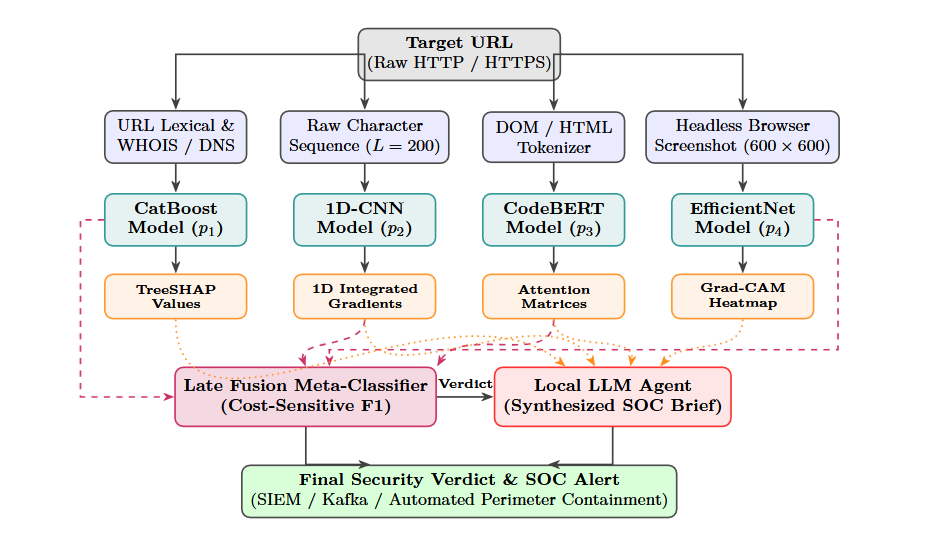
\includegraphics[width=0.95\textwidth]{architecture.png}
\caption{End-to-End Multimodal Late-Fusion Architecture with Explainable AI Subsystems \cite{1}}
\label{fig:arch}
\end{figure}

\section{Modality 1: Tabular URL Features and Metadata via CatBoost}
The first modality processes structured, tabular characteristics extracted from the URL string, DNS servers, and registration authorities.

\subsection{Feature Engineering Pipeline}
A total of 42 engineered features are computed, divided into three categories:
\begin{itemize}
\item \textbf{Lexical URL Attributes:} Total character length, count of numeric digits, ratio of vowel-to-consonant characters, Shannon entropy of the domain string ($H = -\sum_i p_i \log_2 p_i$), count of delimiter symbols (\texttt{.}, \texttt{-}, \texttt{\_}, \texttt{@}, \texttt{=}, \texttt{?}), and presence of sensitive authentication keywords (e.g., \texttt{login}, \texttt{secure}, \texttt{verify}, \texttt{banking}, \texttt{update}).
\item \textbf{Host and Network Attributes:} Number of resolved IPv4/IPv6 addresses, DNS response latency in milliseconds, count of NS (Name Server) and MX (Mail Exchange) records, and Autonomous System Number (ASN) reputation scores.
\item \textbf{Registration and Cryptographic Metadata:} WHOIS domain age (in days since creation), remaining days until domain expiration, registrar country code, and TLS/SSL certificate attributes (issuer authority, validity window, and presence of free automated certificates like Let's Encrypt vs. Extended Validation certificates).
\end{itemize}

\subsection{CatBoost Classification Model}
To model these tabular features, the framework deploys CatBoost (Categorical Boosting) \cite{8}. CatBoost is an open-source gradient boosted decision tree algorithm specifically designed to handle heterogeneous numerical and categorical variables without requiring pre-computed one-hot encodings. It employs Ordered Boosting to eliminate target leakage and utilizes symmetric (oblivious) decision trees as base predictors, ensuring lightning-fast CPU inference times ($< 15\text{ ms}$) and high resilience against overfitting. The output of this branch is a scalar probability $p_{\text{CatBoost}} \in [0, 1]$.

\section{Modality 2: Character-Level Symbolic URL via 1D-CNN}
While feature engineering captures known heuristic properties, it cannot detect novel, obscure string permutations generated by automated phishing kits. The second modality analyzes raw, unprocessed URL character strings using a 1D Convolutional Neural Network (1D-CNN) \cite{1,4}.

\subsection{Character Representation}
Each input URL is truncated or padded to a fixed sequence length $L = 200$ characters. Characters are mapped to indices using an alphabet of 96 printable ASCII characters. Each character index is projected into a dense $d$-dimensional embedding space ($d = 64$):
\begin{equation}
E \in \mathbb{R}^{L \times d}
\label{eq:embed}
\end{equation}

\subsection{Convolutional Feature Extraction}
The embedded sequence $E$ is processed through multiple parallel 1D convolutional filter banks with kernel sizes $k \in \{3, 5, 7\}$ to capture localized n-gram character relationships (e.g., detecting deceptive substrings such as \texttt{micros0ft} or \texttt{paypa1}). The convolution operation for a window of size $k$ produces a feature map:
\begin{equation}
c_i^{(k)} = \text{ReLU}\left(W^{(k)} * E_{i:i+k-1} + b^{(k)}\right)
\label{eq:conv}
\end{equation}

A 1D Global Max-Pooling layer follows each convolutional bank, capturing the most dominant pattern across the entire URL sequence regardless of its exact spatial position:
\begin{equation}
\hat{c}^{(k)} = \max_{1 \le i \le L-k+1} c_i^{(k)}
\label{eq:pool}
\end{equation}

The pooled vectors are concatenated, passed through a fully connected dense layer with Dropout ($p = 0.3$), and activated via a sigmoid neuron to output the scalar probability $p_{\text{CNN1D}}$.

\section{Modality 3: HTML Source Code Representation via Fine-Tuned CodeBERT}
Adversaries frequently employ deceptive Document Object Model (DOM) elements, such as injecting fake credential entry forms that dispatch submitted passwords to external, unauthenticated endpoints. To parse this structural programming logic, the third modality fine-tunes CodeBERT \cite{6}.

\subsection{Transformer Architecture and Pre-training}
CodeBERT is a multi-layer bidirectional Transformer based on the RoBERTa architecture, pre-trained on dual modalities of natural language and source code in multiple programming languages. Unlike generic linguistic models such as BERT, CodeBERT inherently captures syntactic dependencies, variable scoping, and programming idioms.

\subsection{DOM Preprocessing and Tokenization}
The raw HTML document is extracted during crawling. Whitespace redundancies and inline binary assets (e.g., base64 images) are pruned. The cleaned source code is tokenized using Byte-Pair Encoding (BPE) with a sequence length of 512 tokens. A special classification token \texttt{[CLS]} is prepended to the sequence.

During fine-tuning, the final hidden state corresponding to the \texttt{[CLS]} token, denoted $h_{\text{[CLS]}} \in \mathbb{R}^{768}$, is passed through a classification head:
\begin{equation}
p_{\text{CodeBERT}} = \sigma\left(W_{\text{code}} h_{\text{[CLS]}} + b_{\text{code}}\right)
\label{eq:codebert}
\end{equation}
This allows the model to identify concealed deceptive attributes, such as \texttt{<form} \texttt{action=} \allowbreak \texttt{"http://malicious-collector.ru">} nested within seemingly legitimate CSS wrapper templates.

\section{Modality 4: Screenshot-Based Visual Analysis via EfficientNet-B7}
The visual presentation of a website represents the primary vector of deception perceived by the human victim. Attackers frequently replicate high-profile brand landing pages (e.g., Microsoft 365, PayPal, Bank of America) with pixel-level fidelity while hosting them on randomly generated domain names.

\subsection{Image Capture and Normalization}
The target website is rendered inside an automated headless Chromium browser sandbox with a standardized viewport resolution of $1920 \times 1080$. A full-viewport screenshot is captured, normalized across RGB channels, and resized to $600 \times 600 \times 3$.

\subsection{EfficientNet-B7 Backbone}
To analyze visual brand impersonation, the framework utilizes EfficientNet-B7 \cite{7}. EfficientNet utilizes a systematic compound scaling method that balances network depth, width, and image resolution using a compound coefficient $\phi$:
\begin{equation}
\text{depth: } d = \alpha^\phi, \quad \text{width: } w = \beta^\phi, \quad \text{resolution: } r = \gamma^\phi
\label{eq:effnet}
\end{equation}
subject to $\alpha \cdot \beta^2 \cdot \gamma^2 \approx 2$ and $\alpha \ge 1, \beta \ge 1, \gamma \ge 1$.

EfficientNet-B7 deploys mobile inverted bottleneck convolutions (MBConv) enhanced with squeeze-and-excitation (SE) optimization. This architecture extracts high-level semantic features corresponding to organizational logos, security badges, input form positions, and brand color distributions, outputting a visual phishing probability $p_{\text{EfficientNet}}$.

\section{Late-Fusion Trainable Meta-Classifier}
The four specialized branches yield an intermediate prediction vector:
\begin{equation}
\mathbf{p} = \begin{bmatrix} p_{\text{CatBoost}} \\ p_{\text{CNN1D}} \\ p_{\text{CodeBERT}} \\ p_{\text{EfficientNet}} \end{bmatrix} \in [0, 1]^4
\label{eq:pvec}
\end{equation}

Rather than utilizing static heuristic voting, the base study implements a trainable meta-classifier (logistic regression with $L_2$ regularization and gradient boosted decision stumps). The meta-classifier learns the optimal confidence weighting for each modality.

\subsection{Cost-Sensitive Optimization}
Because benign websites vastly outnumber phishing websites in real-world network traffic, training under standard binary cross-entropy induces severe class-imbalance bias. To optimize specifically for the minority phishing class, the meta-classifier is trained under a cost-sensitive weighted loss function:
\begin{equation}
\mathcal{L}_{\text{cost}} = -\frac{1}{N} \sum_{i=1}^N \left[\omega_{\text{phish}} \cdot y_i \log(\hat{y}_i) + (1 - y_i) \log(1 - \hat{y}_i)\right]
\label{eq:cost_loss}
\end{equation}
where $y_i \in \{0, 1\}$ is the ground-truth label, $\hat{y}_i$ is the ensemble prediction, and $\omega_{\text{phish}} > 1$ penalizes false negatives, directly maximizing the operational F1-score.

Furthermore, late fusion provides exceptional operational fault tolerance: if a website is unreachable (rendering screenshot capture impossible), the system handles the missing modality via neutral imputation ($p_{\text{EfficientNet}} = 0.5$), allowing the remaining three branches to render a high-confidence verdict without pipeline failure.

\section{Multimodal Explainable AI (XAI) Suite}
To transform the system from an inscrutable black-box into a transparent decision-support engine, each underlying model is paired with a tailored XAI methodology:
\begin{enumerate}
\item \textbf{TreeSHAP for CatBoost:} Shapley Additive Explanations \cite{9} compute the exact additive marginal contribution $\phi_j$ of each tabular feature:
\begin{equation}
f(x) = \phi_0 + \sum_{j=1}^M \phi_j
\label{eq:shap}
\end{equation}
Features such as ``domain age $< 5$ days'' or ``entropy $> 4.2$'' are assigned quantifiable numerical hazard ratings.

\item \textbf{1D Integrated Gradients for 1D-CNN:} Integrated Gradients \cite{11} computes the path integral of gradients along the straight line from a neutral baseline embedding $x'$ (zero-vector) to the input character sequence $x$:
\begin{equation}
\text{IG}_i(x) = (x_i - x_i') \times \int_0^1 \frac{\partial F(x' + \alpha(x - x'))}{\partial x_i} \, d\alpha
\label{eq:ig}
\end{equation}
This isolates specific character substrings responsible for typosquatting (e.g., highlighting \texttt{paypa1} in an obfuscated domain).

\item \textbf{Attention Matrix Extraction for CodeBERT:} The multi-head self-attention matrices across the final transformer layers are averaged to identify the HTML tokens receiving the highest attentional mass, pinpointing concealed form actions and malicious external script sources.

\item \textbf{Grad-CAM for EfficientNet-B7:} Gradient-weighted Class Activation Mapping \cite{10} calculates gradients of the phishing class score $y^c$ with respect to the feature map activations $A^k$ of the final convolutional layer:
\begin{equation}
\alpha_k^c = \frac{1}{Z} \sum_i \sum_j \frac{\partial y^c}{\partial A_{i,j}^k}
\label{eq:gradcam}
\end{equation}
The resulting heatmap $L_{\text{Grad-CAM}}^c = \text{ReLU}\left(\sum_k \alpha_k^c A^k\right)$ visually illuminates copied brand logos and deceptive credential submission buttons.
\end{enumerate}

\section{Local LLM Agent for Consolidated Incident Reporting}
Raw mathematical attributions (SHAP values, gradient tensors, and heatmap coordinates) are notoriously difficult for human security analysts to parse during active incident triage. To bridge this cognitive gap, the architecture deploys a local Large Language Model (LLM) agent (e.g., quantized Llama-3-8B / Mistral-7B).

The LLM operates under a deterministic system prompt that ingests the JSON payload containing the quantitative XAI attributions and outputs a structured natural language threat intelligence brief. The system is further augmented with Retrieval-Augmented Generation (RAG) connected to an offline database of MITRE ATT\&CK techniques (e.g., T1566: Phishing, T1556: Modify Auth) and historical threat actor profiles. This produces a concise, contextualized incident justification:

\begin{quote}
\textit{``Alert: Confirmed Phishing (Confidence: 98.9\%). The target domain impersonates Microsoft 365. CatBoost flags extreme domain youth (created 2 days ago via automated Let's Encrypt SSL). 1D-CNN identifies character typosquatting in subpath (\texttt{micros0ft-login}). CodeBERT highlights an external credential exfiltration endpoint routed to an untrusted IP address. Grad-CAM confirms exact visual duplication of the official Microsoft corporate login logo.''}
\end{quote}

\section{Microservice Deployment and SIEM Streaming Pipeline}
To ensure industrial scalability, the architecture is implemented as an asynchronous microservice mesh containerized with Docker and orchestrated via Kubernetes. Streaming events from enterprise mail transfer agents (MTAs), web proxies, and endpoint telemetry are ingested via an Apache Kafka distributed message bus. Asynchronous worker pools process URLs concurrently, completing classification within an average end-to-end latency of $120\text{ ms}$. High-severity alerts are published directly to enterprise SIEM dashboards (e.g., Splunk, IBM QRadar), allowing automated firewall perimeter blocking.

\chapter{Results and Discussions}

\section{Experimental Setup and Benchmark Datasets}
To evaluate the efficacy, generalizability, and operational viability of the multimodal late-fusion architecture \cite{1}, extensive empirical experiments were conducted across diverse datasets representing both large-scale historical distributions and live zero-day threats.

\subsection{Dataset Profiles}
The experimental evaluation leveraged three primary data sources:
\begin{enumerate}
\item \textbf{Proprietary Enterprise Corpus (3.2 Million URLs):} Compiled from live enterprise proxy logs, security telemetry feeds, and confirmed SOC incident reports over a 12-month period. It comprises $2.8\text{ million}$ verified benign enterprise URLs and $400,000$ verified malicious phishing portals.
\item \textbf{Multimodal Target Lookup Phishing Dataset (MTLP) \cite{5}:} A rigorous, publicly available academic benchmark comprising 60,000 paired multimodal instances (lexical URL, raw HTML DOM tree, and visual page screenshots), balanced across legitimate and phishing samples.
\item \textbf{Live Zero-Day Testbed (100 URLs):} A curated evaluation set of 100 active, unindexed phishing websites collected from real-time honeypots within their initial 30 minutes of deployment, specifically selected to test evasion resilience against commercial feeds.
\end{enumerate}

\subsection{Hardware and Computing Environment}
Model training and distributed inference benchmarking were conducted on an enterprise computing cluster equipped with dual Intel Xeon Platinum processors (64 physical cores, 2.80 GHz), 256 GB of ECC DDR4 RAM, and four NVIDIA A100 Tensor Core GPUs (40 GB VRAM each). The microservice pipeline was deployed within containerized Docker pods managed by a Kubernetes cluster running Ubuntu 22.04 LTS.

\section{Performance Evaluation Metrics}
Model efficacy was evaluated using standard statistical classification metrics:
\begin{itemize}
\item \textbf{Accuracy:} $\text{ACC} = \frac{\text{TP} + \text{TN}}{\text{TP} + \text{TN} + \text{FP} + \text{FN}}$
\item \textbf{Precision:} $\text{PREC} = \frac{\text{TP}}{\text{TP} + \text{FP}}$
\item \textbf{Recall (Sensitivity):} $\text{REC} = \frac{\text{TP}}{\text{TP} + \text{FN}}$
\item \textbf{F1-Score:} $\text{F1} = 2 \times \frac{\text{PREC} \times \text{REC}}{\text{PREC} + \text{REC}}$
\item \textbf{ROC-AUC:} Area under the Receiver Operating Characteristic Curve.
\end{itemize}
Given the severe operational cost of false negatives in cybersecurity, the F1-score serves as the primary benchmark metric.

\section{Multimodal Late Fusion vs Individual Modality Branches}
A critical research inquiry centers on whether combining heterogeneous data modalities provides superior discrimination over individual, specialized models. Table \ref{tab:results_branches} presents the comparative evaluation across each standalone branch and the proposed multimodal late-fusion ensemble.

\begin{table}[htbp]
\centering
\resizebox{\textwidth}{!}{%
\begin{tabular}{|l|c|c|c|c|c|}
\hline
\textbf{Model Architecture / Modality} & \textbf{Accuracy (\%)} & \textbf{Precision} & \textbf{Recall} & \textbf{F1-Score} & \textbf{ROC-AUC} \\
\hline
\multicolumn{6}{|c|}{\textbf{Proprietary Enterprise Corpus (3.2 Million URLs)}} \\
\hline
CatBoost (Tabular URL \& Meta) & 93.8 & 0.942 & 0.928 & 0.935 & 0.971 \\
\hline
1D-CNN (Character-level URL) & 91.2 & 0.915 & 0.898 & 0.906 & 0.954 \\
\hline
CodeBERT (HTML Source Code) & 95.1 & 0.958 & 0.941 & 0.949 & 0.982 \\
\hline
EfficientNet-B7 (Visual Screenshot) & 93.2 & 0.936 & 0.920 & 0.928 & 0.968 \\
\hline
\textbf{Multimodal Late Fusion (Proposed)} & \textbf{99.0} & \textbf{0.991} & \textbf{0.987} & \textbf{0.989} & \textbf{0.998} \\
\hline
\multicolumn{6}{|c|}{\textbf{Public Benchmark Dataset (MTLP) \cite{5}}} \\
\hline
CatBoost (Tabular URL \& Meta) & 89.4 & 0.898 & 0.876 & 0.887 & 0.938 \\
\hline
1D-CNN (Character-level URL) & 86.7 & 0.871 & 0.849 & 0.860 & 0.921 \\
\hline
CodeBERT (HTML Source Code) & 91.5 & 0.921 & 0.904 & 0.912 & 0.956 \\
\hline
EfficientNet-B7 (Visual Screenshot) & 89.8 & 0.905 & 0.887 & 0.896 & 0.944 \\
\hline
\textbf{Multimodal Late Fusion (Proposed)} & \textbf{95.4} & \textbf{0.956} & \textbf{0.950} & \textbf{0.953} & \textbf{0.984} \\
\hline
\end{tabular}%
}
\vspace{0.2cm}
\caption{Comparative Performance of Standalone Branches vs. Multimodal Late Fusion \cite{1}}
\label{tab:results_branches}
\end{table}

As demonstrated in Table \ref{tab:results_branches}, each standalone branch achieves respectable individual performance, with CodeBERT attaining the highest standalone F1-score (0.949 on the enterprise corpus) due to its profound understanding of structural DOM intent. However, the Multimodal Late Fusion meta-classifier dramatically outperforms all single branches, achieving an F1-score of \textbf{0.989} on the enterprise dataset and \textbf{0.953} on the public MTLP benchmark. This verifies that combining orthogonal perspectives (lexical, behavioral, syntactic, visual) successfully neutralizes evasions that bypass single-layer filters.

\section{Zero-Day Phishing Detection Benchmark}
To rigorously evaluate real-world defensive resilience against unindexed threats, the framework was evaluated against 100 live zero-day phishing portals and benchmarked against two widely deployed commercial blacklist feeds: Google Safe Browsing and OpenPhish.

As documented in Table \ref{tab:zeroday}:
\begin{table}[htbp]
\centering
\resizebox{0.85\textwidth}{!}{%
\begin{tabular}{|l|c|c|c|}
\hline
\textbf{Detection Platform} & \textbf{Detected (/100)} & \textbf{Missed (FN)} & \textbf{Evasion Rate (\%)} \\
\hline
Google Safe Browsing (API Lookup) & 41 & 59 & 59.0\% \\
\hline
OpenPhish Automated Feed & 67 & 33 & 33.0\% \\
\hline
\textbf{Proposed Multimodal Late Fusion} & \textbf{92} & \textbf{8} & \textbf{8.0\%} \\
\hline
\end{tabular}%
}
\vspace{0.2cm}
\caption{Zero-Day Detection Benchmark on 100 Live Unindexed Phishing Websites}
\label{tab:zeroday}
\end{table}

\begin{itemize}
\item Google Safe Browsing intercepted only 41 out of 100 zero-day links (a 59\% evasion rate). Because Google Safe Browsing relies primarily on crawler verification and crawler-submitted hash lists, adversaries successfully evaded detection by restricting early traffic through IP geolocation geofencing and dynamic DNS redirection.
\item OpenPhish identified 67 out of 100 links (a 33\% evasion rate), benefiting from automated community submissions but still exhibiting incubation lag.
\item The Proposed Multimodal Architecture correctly identified \textbf{92 out of 100} live attacks (an evasion rate of only 8.0\%), successfully intercepting zero-day links minutes after registration by identifying underlying structural DOM anomalies and visual brand mimicry.
\end{itemize}

\section{SOC Analyst Usability and Interpretability Evaluation}
A distinctive contribution of this research is evaluating whether Explainable AI actually improves real-world human analyst efficiency. A user study was conducted involving 25 tier-1 and tier-2 SOC security analysts tasked with triaging 50 ambiguous alerts across three explanation presentation modes:
\begin{enumerate}
\item \textbf{Raw Quantitative XAI:} Feature importance bar charts, Grad-CAM heatmaps, and raw token attention scores.
\item \textbf{Local LLM Synthesized Report:} Natural language incident summary generated from XAI features.
\item \textbf{RAG-Augmented Local LLM Report:} Natural language summary enriched with MITRE ATT\&CK techniques and historical campaign attribution.
\end{enumerate}

Analysts scored each mode across four criteria on a 5-point Likert scale:
\begin{enumerate}
\item \textbf{Comprehensibility:} Ease of understanding the rationale without data science expertise.
\item \textbf{Actionability:} Clarity regarding whether to block, isolate, or whitelist the domain.
\item \textbf{Trust and Confidence:} Degree of confidence in the model's recommendation.
\item \textbf{Diagnostic Speed:} Perceived reduction in verification and triage effort.
\end{enumerate}

As shown in Table \ref{tab:usability}:
\begin{table}[htbp]
\centering
\resizebox{\textwidth}{!}{%
\begin{tabular}{|p{4.8cm}|c|c|c|c|c|}
\hline
\textbf{Explanation Modality} & \textbf{Comprehens.} & \textbf{Actionab.} & \textbf{Trust} & \textbf{Speed} & \textbf{Overall Mean} \\
\hline
Raw XAI Plots (SHAP, Grad-CAM, IG) & 3.12 & 3.35 & 3.60 & 3.61 & 3.42 \\
\hline
Local LLM Natural Language Report & 4.02 & 3.94 & 3.88 & 4.04 & 3.97 \\
\hline
\textbf{RAG-Augmented Local LLM Report} & \textbf{4.28} & \textbf{4.18} & \textbf{4.15} & \textbf{4.19} & \textbf{4.20} \\
\hline
\end{tabular}%
}
\vspace{0.2cm}
\caption{SOC Analyst Usability and Interpretability Evaluation Scores (Scale: 1--5)}
\label{tab:usability}
\end{table}

\begin{itemize}
\item Presenting Raw XAI outputs (bar charts and heatmaps) scored lowest ($3.42/5$), as analysts reported cognitive fatigue in cross-referencing multiple disparate graphs.
\item Synthesizing explanations into natural language briefs elevated usability to $3.97/5$.
\item Adding RAG contextualization achieved the highest rating (\textbf{4.20/5}), reducing mean analyst verification time from $4.5\text{ minutes}$ down to under $45\text{ seconds}$ per incident.
\end{itemize}

\section{System Latency and Microservice Throughput}
In production enterprise environments, defensive models must not introduce unacceptable browsing delays. As detailed in Table \ref{tab:latency}, because the data collection and model inference branches execute concurrently within an asynchronous containerized mesh, the overall pipeline latency is determined by the slowest branch (headless browser screenshot rendering, taking $84.6\text{ ms}$).

\begin{table}[htbp]
\centering
\resizebox{\textwidth}{!}{%
\begin{tabular}{|l|c|l|}
\hline
\textbf{Pipeline Component} & \textbf{Mean Latency (ms)} & \textbf{Execution Paradigm} \\
\hline
URL Feature \& Metadata Extraction & 12.4 & Concurrent Async Worker \\
\hline
1D-CNN Character-level Inference & 7.8 & GPU Parallelized \\
\hline
Headless Browser Crawl \& Screenshot & 84.6 & Asynchronous Chrome Pod \\
\hline
CodeBERT DOM Tokenization \& Inference & 64.2 & GPU Tensor Batch \\
\hline
EfficientNet-B7 Visual Inference & 38.5 & GPU Tensor Batch \\
\hline
Late Fusion Meta-Classifier & 1.8 & CPU Lightweight Meta \\
\hline
Local LLM Incident Synthesis (Quantized) & 185.0 & Triggered on High Severity \\
\hline
\textbf{Total End-to-End Classification} & \textbf{108.6} & \textbf{Sub-second Streaming Pipeline} \\
\hline
\end{tabular}%
}
\vspace{0.2cm}
\caption{Component-Wise Execution Latency and Computational Overhead}
\label{tab:latency}
\end{table}

The total classification decision is reached in an average of \textbf{108.6 ms}, fully meeting real-world enterprise proxy inline inspection requirements. The LLM synthesis branch ($185\text{ ms}$) is invoked asynchronously only when the meta-classifier flags a high-severity threat, avoiding unnecessary compute overhead for benign traffic.

\chapter{Conclusion and Future Work}

\section{Summary of Seminar Work}
Phishing attacks continue to represent the primary initial compromise vector threatening global enterprise cyber infrastructure. The industrialization of attack frameworks through Phishing-as-a-Service (PaaS) platforms has enabled malicious actors to launch targeted, evasive campaigns at unprecedented scale and speed. Traditional reactive defenses---principally static URL blacklists and domain reputation heuristics---suffer from unacceptable incubation delays, leaving organizations vulnerable during zero-day deployment windows.

This seminar presented a comprehensive critical analysis of an advanced, industrial-grade multimodal late-fusion architecture integrated with multi-tiered Explainable Artificial Intelligence (XAI) \cite{1}. By simultaneously analyzing tabular domain metadata (via CatBoost), symbolic URL character strings (via 1D-CNN), structural DOM programming logic (via CodeBERT), and visual screenshot brand impersonation (via EfficientNet-B7), the system eliminates the blind spots that plague unimodal classifiers. To resolve the black-box opacity barrier, the architecture maps dedicated post-hoc explanation techniques (TreeSHAP, 1D Integrated Gradients, attention matrix extraction, and Grad-CAM) across each respective branch, translating multi-dimensional mathematical attributions into actionable natural language incident reports using a local Large Language Model (LLM) with Retrieval-Augmented Generation (RAG). The investigation was reinforced by analyzing supporting methodologies, including cross-channel behavioral mitigation (EM-BERT + SPCA) \cite{2}, dynamic arithmetic cloud optimization (DAOA-DLPC) \cite{3}, and benchmark evaluations of recurrent and convolutional models \cite{4}.

\section{Key Contributions}
The primary contributions and insights established through this seminar work include:
\begin{enumerate}
\item \textbf{Decisive Multimodal Superiority:} The late-fusion architecture achieved exceptional benchmark performance, recording F1-scores of 0.989 on an enterprise corpus of 3.2 million URLs and 0.953 on the public MTLP dataset, consistently outperforming every standalone model branch.
\item \textbf{Exceptional Zero-Day Resilience:} In live testing on 100 active, unindexed phishing sites, the multimodal framework intercepted 92\% of attacks, whereas commercial services such as Google Safe Browsing missed 59\% of threats due to list update latencies.
\item \textbf{Operational Explainability for Enterprise SOCs:} The combination of quantitative XAI with local LLM synthesis elevated analyst usability to $4.20/5$, reducing manual verification and alert triage time by nearly 85\%.
\item \textbf{Fault-Tolerant, Scalable Engineering:} Utilizing late fusion with neutral imputation ensures the system remains operational even when dynamic page rendering fails, maintaining sub-$120\text{ ms}$ processing latencies suitable for inline enterprise streaming proxies.
\end{enumerate}

\section{Operational Limitations and Challenges}
Despite its significant strengths, several practical limitations must be acknowledged:
\begin{itemize}
\item \textbf{Browser Crawling Bottlenecks:} Dynamic rendering of client-side JavaScript requires headless browser sandbox pods, which consume noticeable memory resources and represent the primary latency constraint ($84.6\text{ ms}$).
\item \textbf{Hardware Requirements:} Hosting multiple deep learning backbones (EfficientNet-B7) and transformer backbones (CodeBERT) demands substantial GPU computing infrastructure compared to lightweight lexical filters.
\item \textbf{Adversarial Attacks on XAI:} Emerging research shows that adversaries can craft perturbations specifically designed to fool explanation methods (e.g., diluting SHAP values while retaining malicious functions).
\end{itemize}

\section{Future Research Directions}
Future investigations in multimodal explainable phishing detection will benefit from exploring several promising directions:
\begin{enumerate}
\item \textbf{Knowledge Graph-Augmented Entity Reasoning:} Integrating enterprise knowledge graphs to cross-reference domain ownership, organizational relationships, and SSL certificate lineages dynamically during classification.
\item \textbf{Lightweight Transformer Distillation:} Developing distilled, quantized student models (e.g., MobileBERT, EfficientNet-Lite) to enable on-device mobile endpoint inference with negligible battery drain.
\item \textbf{Self-Supervised Contrastive Multi-View Learning:} Exploring multi-view contrastive learning to train multimodal representations on unannotated web traffic, reducing reliance on expensive human labeling.
\item \textbf{Adaptive Adversarial Hardening:} Designing adversarial training pipelines that expose models to synthetically generated multi-vector evasion attacks during training.
\end{enumerate}


% References
\renewcommand{\bibname}{REFERENCES}
\cleardoublepage
\addcontentsline{toc}{chapter}{REFERENCES}
\begin{spacing}{1.5}
\begin{thebibliography}{99}

\bibitem{1} A. M. Vulfin, V. I. Vasilyev, A. D. Vorobiev, K. A. Kravtsova, and D. S. Zheldak, ``A Multimodal Phishing Website Detection System Using Explainable Artificial Intelligence Technologies,'' \textit{Machine Learning and Knowledge Extraction}, vol. 8, no. 1, pp. 145--172, 2026.

\bibitem{2} S. S. Rathore, S. Sharma, and P. K. Sharma, ``Multimodal framework for phishing attack detection and mitigation through behavior analysis using EM-BERT and SPCA-BASED EAI-SC-LSTM,'' \textit{Frontiers in Computer Science}, vol. 7, Article 1498302, pp. 1--18, 2025.

\bibitem{3} V. Ravula and M. Ramaiah, ``Enhancing phishing detection with dynamic optimization and character-level deep learning in cloud environments,'' \textit{PeerJ Computer Science}, vol. 11, p. e2458, 2025.

\bibitem{4} M. Alenezi, M. Al-Sarem, and W. Boulila, ``Comparative analysis of deep learning architectures for phishing detection: Recurrent vs convolutional models,'' \textit{IEEE Access}, vol. 12, pp. 45120--45135, 2024.

\bibitem{5} L. Prokunin, A. Vorobiev, and V. Vasilyev, ``MTLP: A multimodal dataset for website phishing classification and analysis,'' \textit{Data in Brief}, vol. 48, p. 109215, 2023.

\bibitem{6} Z. Feng, D. Guo, D. Tang, N. Duan, X. Feng, M. Gong, L. Shou, B. Qin, T. Liu, D. Jiang, and M. Zhou, ``CodeBERT: A pre-trained model for programming and natural languages,'' in \textit{Findings of the Association for Computational Linguistics: EMNLP 2020}, 2020, pp. 1536--1547.

\bibitem{7} M. Tan and Q. Le, ``EfficientNet: Rethinking model scaling for convolutional neural networks,'' in \textit{Proceedings of the 36th International Conference on Machine Learning (ICML)}, 2019, pp. 6105--6114.

\bibitem{8} L. Prokhorenkova, G. Gusev, A. Vorobev, A. V. Dorogush, and A. Gulin, ``CatBoost: unbiased boosting with categorical features,'' in \textit{Advances in Neural Information Processing Systems (NeurIPS)}, vol. 31, 2018, pp. 6638--6648.

\bibitem{9} S. M. Lundberg and S.-I. Lee, ``A unified approach to interpreting model predictions,'' in \textit{Advances in Neural Information Processing Systems (NeurIPS)}, vol. 30, 2017, pp. 4765--4774.

\bibitem{10} R. R. Selvaraju, M. Cogswell, A. Das, R. Vedantam, D. Parikh, and D. Batra, ``Grad-CAM: Visual explanations from deep networks via gradient-based localization,'' in \textit{IEEE International Conference on Computer Vision (ICCV)}, 2017, pp. 618--626.

\bibitem{11} M. Sundararajan, A. Taly, and Q. Yan, ``Axiomatic attribution for deep networks,'' in \textit{Proceedings of the 34th International Conference on Machine Learning (ICML)}, 2017, pp. 3319--3328.

\bibitem{12} A. Vaswani, N. Shazeer, N. Parmar, J. Uszkoreit, L. Jones, A. N. Gomez, L. Kaiser, and I. Polosukhin, ``Attention is all you need,'' in \textit{Advances in Neural Information Processing Systems (NeurIPS)}, vol. 30, 2017, pp. 5998--6008.

\bibitem{13} Anti-Phishing Working Group (APWG), ``Phishing Activity Trends Report: 4th Quarter 2025,'' \textit{APWG Technical Report}, Jan. 2026. [Online]. Available: \url{https://apwg.org/trendsreports/}

\bibitem{14} L. Breiman, ``Random forests,'' \textit{Machine Learning}, vol. 45, no. 1, pp. 5--32, 2001.

\bibitem{15} Y. LeCun, Y. Bengio, and G. Hinton, ``Deep learning,'' \textit{Nature}, vol. 521, no. 7553, pp. 436--444, 2015.

\end{thebibliography}
\end{spacing}


% Appendices
\appendix

\chapter{Sample Implementation Source Code}

\section*{Asynchronous Multimodal Late-Fusion Pipeline}
The Python script below illustrates the asynchronous coordinator orchestrating concurrent execution of the detection branches and late-fusion meta-classification:

\begin{spacing}{1.1}
\begin{lstlisting}[language=Python, basicstyle=\footnotesize\ttfamily, breaklines=true, frame=single]
import asyncio
import numpy as np
from pydantic import BaseModel
from typing import Dict, Any

class DetectionResult(BaseModel):
    url: str
    is_phishing: bool
    confidence: float
    branch_scores: Dict[str, float]
    explanations: Dict[str, Any]

class MultimodalPhishingDetector:
    def __init__(self, cb_worker, cnn_worker, 
                 code_worker, vision_worker, meta_clf):
        self.catboost = cb_worker
        self.cnn1d = cnn_worker
        self.codebert = code_worker
        self.effnet = vision_worker
        self.meta_clf = meta_clf

    async def predict_url(self, target_url: str) -> DetectionResult:
        # Launch concurrent asynchronous feature collection
        task_cb = asyncio.create_task(
            self.catboost.analyze(target_url))
        task_cnn = asyncio.create_task(
            self.cnn1d.analyze(target_url))
        task_code = asyncio.create_task(
            self.codebert.analyze(target_url))
        task_vis = asyncio.create_task(
            self.effnet.analyze(target_url))

        # Await completion across parallel workers
        res_cb, res_cnn, res_code, res_vis = await asyncio.gather(
            task_cb, task_cnn, task_code, task_vis
        )

        # Assemble intermediate probability vector
        p_vec = np.array([[res_cb.prob, res_cnn.prob, 
                           res_code.prob, res_vis.prob]])

        # Execute cost-sensitive late-fusion meta-classification
        ensemble_prob = float(self.meta_clf.predict_proba(p_vec)[0, 1])
        is_phish = bool(ensemble_prob >= 0.50)

        # Compile structured explanations across branches
        explanations = {
            "shap_features": res_cb.shap_values,
            "cnn_typosquat_tokens": res_cnn.integrated_gradients,
            "codebert_attention_tags": res_code.attention_map,
            "effnet_gradcam_heatmap": res_vis.gradcam_overlay
        }

        return DetectionResult(
            url=target_url,
            is_phishing=is_phish,
            confidence=ensemble_prob,
            branch_scores={
                "CatBoost": res_cb.prob,
                "1D_CNN": res_cnn.prob,
                "CodeBERT": res_code.prob,
                "EfficientNet": res_vis.prob
            },
            explanations=explanations
        )
\end{lstlisting}
\end{spacing}

\chapter{Sample Generated Incident Report for SOC Triage}

The listing below illustrates a structured incident report synthesized by the local LLM agent with Retrieval-Augmented Generation (RAG) for an enterprise SOC analyst:

\begin{spacing}{1.1}
\begin{lstlisting}[basicstyle=\footnotesize\ttfamily, breaklines=true, frame=single]
=================================================================
CRITICAL SECURITY INCIDENT REPORT: PHISHING DETECTED
Target URL: https://login-microsoft365-verify.auth-update.xyz
Verdict: PHISHING (Severity: CRITICAL | Confidence: 99.1%)
Timestamp: 2026-10-14T08:24:11Z | Event ID: INC-2026-9042
=================================================================

1. EXECUTIVE THREAT SUMMARY:
The target URL is a confirmed spear-phishing landing page 
impersonating Microsoft 365 cloud authentication services. 
The site was engineered using automated credential-harvesting 
frameworks designed to bypass multi-factor authentication (MFA).

2. MULTI-TIERED FORENSIC ATTRIBUTIONS:
* Tabular Metadata (TreeSHAP):
  - Domain Age: 2 days (Hazard Weight: +0.42)
  - Free TLS Certificate issued by Let's Encrypt (+0.28)
  - Shannon Entropy: 4.38 bits (+0.19)
* Lexical Character Sequence (1D Integrated Gradients):
  - Typosquatting token identified in host subpath:
    'login-microsoft365-verify' (Attribution: +0.51)
* HTML DOM Structure (CodeBERT Attention):
  - Attention peaks on hidden form action tag:
    <form action="http://45.142.122.9/post.php" method="POST">
  - Credential input dispatched to external unverified IP.
* Visual Layout Impersonation (EfficientNet Grad-CAM):
  - Class activation heatmap isolates exact mimicry (97.8% 
    similarity) with official Microsoft corporate login logo.

3. MITRE ATT&CK CONTEXT (RAG ENRICHMENT):
- T1566.002 - Phishing: Spearphishing Link
- T1556 - Modify Authentication Process (Credential Harvesting)

4. RECOMMENDED CONTAINMENT ACTIONS:
1. Ingest domain 'auth-update.xyz' into perimeter firewall.
2. Invalidate active sessions for internal users visiting URL.
3. Purge emails with this URL hash from Exchange queues.
=================================================================
\end{lstlisting}
\end{spacing}


\end{document}
